% Template for Cogsci submission with R Markdown

% Stuff changed from original Markdown PLOS Template
\documentclass[10pt, letterpaper]{article}

\usepackage{cogsci}
\usepackage{pslatex}
\usepackage{float}
\usepackage{caption}

% amsmath package, useful for mathematical formulas
\usepackage{amsmath}

% amssymb package, useful for mathematical symbols
\usepackage{amssymb}

% hyperref package, useful for hyperlinks
\usepackage{hyperref}

% graphicx package, useful for including eps and pdf graphics
% include graphics with the command \includegraphics
\usepackage{graphicx}

% Sweave(-like)
\usepackage{fancyvrb}
\DefineVerbatimEnvironment{Sinput}{Verbatim}{fontshape=sl}
\DefineVerbatimEnvironment{Soutput}{Verbatim}{}
\DefineVerbatimEnvironment{Scode}{Verbatim}{fontshape=sl}
\newenvironment{Schunk}{}{}
\DefineVerbatimEnvironment{Code}{Verbatim}{}
\DefineVerbatimEnvironment{CodeInput}{Verbatim}{fontshape=sl}
\DefineVerbatimEnvironment{CodeOutput}{Verbatim}{}
\newenvironment{CodeChunk}{}{}

% cite package, to clean up citations in the main text. Do not remove.
\usepackage{apacite}

% KM added 1/4/18 to allow control of blind submission


\usepackage{color}

% Use doublespacing - comment out for single spacing
%\usepackage{setspace}
%\doublespacing


% % Text layout
% \topmargin 0.0cm
% \oddsidemargin 0.5cm
% \evensidemargin 0.5cm
% \textwidth 16cm
% \textheight 21cm

\title{Modeling Selection in Active Cross-situational Word Learning}


\author{{\large \bf George~Kachergis (kachergis@stanford.edu)} \\ Department of Psychology, Stanford University \\ Stanford, CA \AND {\large \bf Martin~Zettersten (mzettersten@ucsd.edu)} \\ Department of Cognitive Science, University of California, San Diego \\ San Diego, CA}

\newlength{\cslhangindent}
\setlength{\cslhangindent}{1.5em}
\newenvironment{CSLReferences}%
  {}%
  {\par}

\begin{document}

\maketitle

\begin{abstract}
Word learning is a complex, interactive process, in which learners do
not passively observe a stream of words and referents, but are rather
actively involved in selecting referents and directing their attention
-- both of which are likely determined by their current knowledge state.
Thus, understanding how learners actively select information during word
learning can reveal the cognitive mechanisms underlying language
acquisition. The present study reanalyzes data from Zettersten \&
Saffran (2021), in which adults and children (ages 3-8) learned novel
word-referent mappings through cross-situational learning, then selected
which referents to receive additional training on. Participants'
individual training data, selection choices, and test trials were used
to fit four associative word learning models, and to infer the most
likely of five sampling strategies. Models with a bias to attend to
stimuli with uncertain (i.e.~high-entropy) knowledge states best
accounted for the data, although \textasciitilde51\% participants appear
to be driven solely by this bias, while another 48\% apparently also
engage a competing familiarity bias. Analysis of selection strategies
revealed developmental differences: adults often used entropy
maximization (39\% of adults vs.~20\% of children) to reduce uncertainty
about ambiguous items, while children favored confirmatory sampling
(62\% vs.~22\% of adults), seeking information about items with
established associations. These findings suggest that the ability to
strategically sample ambiguous information develops gradually, and that
individual differences in learning mechanisms---particularly learning
rate and memory---are more predictive of word learning success than
sampling strategy alone.

\textbf{Keywords:}
active learning; cross-situational word learning; self-directed
learning; uncertainty reduction
\end{abstract}

\section{Introduction}\label{introduction}

Early word learning is often viewed as largely determined by the
learner's linguistic environment, where acquisition is constrained by
what is present in the input. Increasingly, however, research reveals
that learners--even young children--actively select and shape their
input, and that such self-directed learning can accelerate acquisition
(Smith, Jayaraman, Clerkin, \& Yu, 2018; Twomey \& Westermann, 2018).
Understanding the strategies learners use to curate their experience can
advance theories of language acquisition, reveal the cognitive
mechanisms and capacities available across development, and inform the
design of educational curricula that match learners' expanding
capabilities.

Despite growing interest in active learning, most computational models
of word learning have been evaluated exclusively on passive
cross-situational learning paradigms, in which participants observe
ambiguous training trials presenting multiple word-referent pairs
without indication of the correct mappings (G. Kachergis, Yu, \&
Shiffrin, 2016; Yu \& Smith, 2007). While model comparisons in these
passive contexts are informative, active learning paradigms in which
learners control some aspect of their input (e.g., selecting which item
to learn about next) can be more diagnostic of underlying learning
mechanisms and may better capture individual differences in learning
success (Gureckis \& Markant, 2012; Markant, Settles, \& Gureckis,
2016). Yet few active word learning experiments have been conducted, and
fewer still have attempted to explain active learning behavior with
computational models (though see George Kachergis, Yu, \& Shiffrin,
2013).

The goal of the current study is to test how well associative models of
cross-situational word learning can explain both learning outcomes and
sampling strategies in the active learning experiments of Zettersten \&
Saffran (2021). In those experiments, adults preferentially selected
items with ambiguous word-referent mappings during a sampling phase,
while children (ages 3-8) did not show this preference. We address three
main questions: First, which model architecture best captures individual
learning performance? Second, do specific model parameters (learning
rate, memory decay, attention to uncertainty) predict learning success?
To address these first two issues, we chose a family of models that
instantiate trial-by-trial associative learning with memory decay and
selective attention to familiar and/or uncertain (or novel) stimuli,
which have been shown to account well for semantic bootstrapping and
mutual exclusivity effects in prior work (G. Kachergis et al., 2016; Y.
Kachergis G., 2012). Third, what sampling strategies (e.g., information
gain, confirmatory sampling, margin sampling) best explain participants'
information-seeking choices, and how do these strategies develop with
age?

Understanding children's and adults' sampling strategies during word
learning has important implications for theories of vocabulary
development. Past work shows that both children and adults actively seek
information about word meanings (Hembacher, DeMayo, \& Frank, 2020),
which may help explain rapid vocabulary growth (Hidaka, Torii, \&
Kachergis, 2017). However, we lack a formal understanding of the
specific decision rules governing when learners seek new information
versus consolidate existing knowledge (Settles, 2012; though see
Gelderloos, Mahmoudi Kamelabad, \& Alishahi, 2020; Keijser, Gelderloos,
\& Alishahi, 2019). Recent developmental work documents broad changes in
information-seeking strategies across childhood in domains such as
causal learning (Nussenbaum et al., 2019) and foraging (Meder, Wu,
Schulz, \& Ruggeri, 2021; Nussenbaum et al., 2023), suggesting that
strategic sampling may emerge gradually with age and cognitive
development. The current work therefore explores what sampling decision
rules best explain children's and adults' information-seeking during
word learning, and how learning mechanisms relate to sampling
strategies.

A central theoretical question concerns the relationship between
learning success and sampling strategy. Zettersten \& Saffran (2021)
found that adults who sampled more ambiguous items during the selection
phase showed higher test accuracy. However, the directionality of this
relationship remains unclear: does sampling ambiguous items \emph{cause}
better learning, or does successful learning \emph{enable} more
sophisticated ambiguity-seeking strategies? Their supplementary analyses
suggested the latter: as participants became more successful at learning
during training, they became more likely to seek information about
ambiguous items. We investigate this question by examining whether
individual differences in learning parameters (learning rate, memory,
attention biases) predict both test performance and sampling strategy,
potentially illuminating the mechanisms linking learning capacity to
active information-seeking.

\section{Method}\label{method}

\subsection{Data}\label{data}

All data were taken from Zettersten \& Saffran (2021). Data for our
Study 1 were pooled from Experiment 1 (31 adults), Experiment 2 (40
children, 4-9 years of age), and adults in the Ambiguous Condition of
Experiment S1 (58 adults), which had the same design as Experiments 1
and 2, except for an additional test before the selection phase. The
training phase of Study 1 contained 24 trials, each comprised of 2
referents and 2 words. The particular words and referents involved in
each pairing were randomized per participant, but the same training
trial sequence--and thus co-occurrence statistics--were experienced by
all participants.

Data for Study 2 come from Experiment 3, comprising 58 children, 3 to 8
years of age.

Selection trials for kids differ slightly from adults in that there was
no random label-referent pair given: thus, the evidence children
received after selection was unambiguous, while adults received a
training trial with a randomly-selected label and its corresponding
referent. The models will see what the learner saw: for children, that
would be an unambiguous trial with the selected referent and its label;
while for adults, the model will be presented with the selected stimulus
pair alongside the random pair the learner saw.

\subsection{Models}\label{models}

We focused on analyzing data from the familiarity- and
uncertainty-biased associative model G. Kachergis et al. (2016), and
variations of that model, described below. We chose not to test any
hypothesis-testing (HT) model as they are not consistent with the adult
data in Zettersten \& Saffran (2021): for ambiguous items in the
training phase, there was never any disconfirming evidence, so a
hypothesis-tester's initial guess (i.e.~hypothesis) for each label would
be confirmed on subsequent appearances, and there would be no reason for
(or basis for) preferentially selecting ambiguous referents during the
sampling phase, which is what adults were observed to do. While it is
possible that children -- who were at chance for selecting ambiguous
vs.~unambiguous referents -- are employing a hypothesis-testing
strategy, some of the selection strategies we want to evaluate across
development are only possible to use if a learner is simultaneously
entertaining multiple hypotheses for a given label -- equivalent to
associations rather than the mutually-exclusive hypotheses favored in HT
accounts (e.g. Woodard, Gleitman, \& Trueswell, 2016).

\subsubsection{Familiarity- and Uncertainty-biased Associative Model
(FUAM)}\label{familiarity--and-uncertainty-biased-associative-model-fuam}

The FUAM assumes that learners accumulate associations between all
presented words and referents on each trial, but that their attention is
biased more towards particular word-referent associations on the basis
of prior experience. In particular, more attention (i.e.~associative
weight) is directed to associations between words and referents that
have appeared together on earlier trials (i.e., a familiarity bias). In
addition, more attention is directed to stimuli that have higher
uncertainty (i.e.~entropy, \(H\)) in their associations, whether because
they are novel (and thus have no pre-existing associations) or because
they have diffuse associations with several different stimuli. The model
assumes learners knowledge grows trial-by-trial, and that a fixed amount
of associative weight (learning rate \(\chi\)) is distributed among the
presented word-referent associations on a given trial in proportion to
the prior familiarity of the association and the uncertainty of the
involved word and referent. The relative strength of the familiarity and
uncertainty bias is governed by a parameter \(\lambda\): for values of
\(\lambda>1\) the model focuses more attention on uncertain stimuli,
while for values of \(\lambda<1\) the model focuses more attention on
familiar word-referent associations. Associations are also assumed to
decay from trial to trial, at a rate governed by memory fidelity
parameter \(\alpha\). The update rule for adjusting the association
\(M_{w,o}\) between word \(w\) and referent \(o\) on a given trial is

\begin{equation}
M_{w,o} =  \alpha M_{w,o} + \frac{ \chi \cdot e^{ \lambda \cdot (H(w) + H(o)) } \cdot M_{w,o}  }{  \sum_{w\in W} \sum_{o\in O} e^{ \lambda \cdot (H(w) + H(o)) } \cdot M_{w,o} }
\label{eq:fullmodel}
\end{equation}

When tested on word \(w\), the model assumes learners choose referent
\(o\) from the offered alternatives in proportion to their associative
strength \(M_{w,o}\) (i.e., Luce choice).

The other models we tested are variations on this model.

\subsubsection{Familiarity-biased Associative Model
(FAM)}\label{familiarity-biased-associative-model-fam}

The familiarity-biased associative model (FAM) implemented just the
familiarity bias of the FUAM, without the uncertainty bias term, and
thus only implements a bias for already-strong associations, using
learning rate (\(\chi\)) and decay \(\alpha\) parameters.

\subsubsection{Uncertainty-biased Associative Model
(UAM)}\label{uncertainty-biased-associative-model-uam}

The uncertainty-biased associative model (UAM) implemented only the
uncertainty bias of the FUAM, without the familiarity bias term, and
uses the same three parameters as the FUAM.

\subsubsection{Novelty-biased Associative Model
(NAM)}\label{novelty-biased-associative-model-nam}

The novelty-biased associative model (NAM), like the UAM, has no
familiarity bias, but instead of the entropy terms (\(H(w)\) and
\(H(o)\)) uses novelty (e.g., \(1/(frequency(w)+1)\)).

\subsection{Fitting Procedure}\label{fitting-procedure}

We first fitted each model to each participant's data individually,
finding parameter values per participant to maximize the log-likelihood
of the model's choices with respect to theirs. We fitted each model to
just the passive training trials, as well as to the passive training
trials and the participant's selection trials, to confirm that including
the selection trials yielded a better fit. We will report each model's
average fit, and select the best-fitting model overall for further
analysis.

\subsection{Modeling Sampling Choices}\label{modeling-sampling-choices}

Next, we used the best-fit models of participants' learning to
investigate their selection strategies in the sampling phase of the
experiment. We considered three sampling decision rules commonly
attested in the information-seeking literature to explain active
choices: maximizing entropy reduction (information gain), maximizing the
probability associated with labels (probability gain), and margin
sampling.

\subsubsection{Maximizing entropy
reduction.}\label{maximizing-entropy-reduction.}

In this decision rule, the model's goal is to maximally reduce the
entropy of the object-label probability distribution across objects
(Nelson, 2005; Settles, 2012). Sampling choices are modeled based on
comparing the relative entropy reduction provided by making a given
sampling selection of a referent \(s_o\) (across the labels \(w\)):

\begin{equation}
\max_{s_o,w}({H(w)-H(w|s_o)})
\label{eq:entropy_reduction}
\end{equation}

Modeling selections were made by determining, on any given trial for a
participant, which object maximally reduced entropy (averaging across
all possible random distractors that could be chosen in the case of the
adult data).

\subsubsection{Margin sampling.}\label{margin-sampling.}

An alternative strategy documented in describing active sampling
strategies is focusing on reducing uncertainty for a more constrained
set of items (Markant et al., 2016). This strategy can be formalized as
\emph{margin sampling}, in which the model focuses only on the boundary
between two alternative options. Margin sampling predicts that learners
will focus on instances where there is highest ambiguity between the two
most likely labels for a given referent. Formally, if the distribution
of labels (\(\{l_1,l_2,...,l_n\}\)) for a given referent \(o\) are
ordered from most (\(p_1\)) to least (\(p_n\)) likely,
\(\{p_1,p_2,...,p_n\}\), the margin between labels is given by

\begin{equation}
LM(x) = 1 - (p_1 - p_2)
\label{eq:margin_sampling}
\end{equation}

In other words, the model selects the object that has the greatest
ambiguity or competition between its two strongest associates.

\subsubsection{Maximizing probability
gain.}\label{maximizing-probability-gain.}

In this decision rule, the model's goal is to maximally increase the
probability associated between a random label and its object (Nelson,
McKenzie, Cottrell, \& Sejnowski, 2010). Selection choices are modeled
based on determining the increase in (correct) association strength
provided by a each potential object selection. The final object was
selected that led to the largest increase in association strength
(averaging across all possible distractors that could be chosen in the
case of the adult data).

\begin{equation}
\max_{s_o,w}({M_{w,s_o})- \max_{w,o}(M_{w,o}})
\label{eq:probability_gain}
\end{equation}

\subsubsection{Alternative strategies.}\label{alternative-strategies.}

We also explored several additional strategies. First, we also
considered a \emph{maximum certainty} (or confirmatory) strategy.
Learners may gravitate towards confirming choices they already have high
certainty for (Wason, 1960; Zettersten, Cutler, \& Lew-Williams, 2023).
Second, we considered a \emph{novelty-based} strategy in which the model
based its choices on the relative novelty (or familiarity) of the choice
options. Third, we consider a random selection strategy as a baseline
comparison.

\section{Results}\label{results}

\begin{table}[H]
\centering
\begin{tabular}{lrrrrr}
  \hline
Model & N best fit & Fam & Unc & Nov & FUAM \\
  \hline
FUAM &  67 & 1.66 & 1.66 & 1.65 & 1.42 \\
  Fam &  24 & 2.00 & 2.09 & 2.00 & 2.00 \\
  Nov &   3 & 3.22 & 3.42 & 3.01 & 3.19 \\
  Unc &  96 & 3.56 & 2.57 & 3.49 & 3.37 \\
   \hline
\end{tabular}
\caption{Number of participants best fitted per model, and average negative log-likelihood (lower=better) per model.}
\end{table}

For all four models, including the selection trials yielded a better fit
to the data, showing that it is not unreasonable to apply these models
to the selection trials, and supporting the idea that the model's
knowledge state and parameters may bear some relation to participants'
selection strategies. For model comparison, we calculated BIC (Bayesian
Information Criterion), defined as \(BIC=ln(N)k-2ln(L)\), where \(L\) is
the maximized likelihood, \(k\) is the number of parameters, and \(N\)
is the number of data points (here, \(N=1712\) test trials). The model
with the lowest BIC is selected, as it balances model complexity and fit
to the data. The familiarity-biased model yielded \(BIC = 1036.17\), the
novelty-biased model scored \(BIC = 1026.68\), and the familiarity- and
uncertainty-biased model (FUAM) had \(BIC = 975.22\). The
uncertainty-biased model (UAM) yielded the best fit, with
\(BIC = 859.09\). Recognizing that different participants may be
operating under different learning regimes, we opted to investigate how
many participants were best fitted by each model. The uncertainty-biased
model best matched behavior of 96 of the 190 participants (51\% of the
sample), and the average fit (negative log-likelihood; see Table 1) of
the model to its best-fitted participants was much better (i.e.~lower)
than any other model (2.57 vs.~3.37 by the FUAM model). The FUAM
achieved the best fit for 67 participants, with the best average fit to
that group seen in Table 1 (1.42). The FUAM also matched the best fit of
the familiarity-biased model to 3 decimal places (see Table 1) for the
24 participants that were best fitted by that model, making for a total
of 91 participants (48\% of the sample) that are best or nearly equally
well accounted for by the FUAM model (the uncertainty model did not fit
as well to the strength participants). The novelty-biased model best
fitted only 3 participants, although it's worth noting that its average
fit to the strength participants was nearly the same as the FUAM and
strength models. We will focus our remaining analyses on the model
parameters for the two best-fitting models, the familiarity- and
uncertainty-biased associative model (FUAM) and its cousin the
uncertainty-biased associative model (UAM).

\subsection{Model parameters}\label{model-parameters}

The FUAM and UAM models achieved similar fit
(\(|NLL_{FUAM} - NLL_{UAM}| \leq 0.1\)) for 98 participants. The UAM
achieved better fit than the FUAM (\(NLL_{FUAM} - NLL_{UAM} > 0.1\)) for
56 participants, and the FUAM achieved better fit than the UAM for the
remaining 36 participants. We will call these participants the
\emph{Either}, \emph{UAM}, and \emph{FUAM} groups, respectively.

\begin{table}[H]
\centering
\begin{tabular}{lrrrrr}
  \hline
Group & N & chi & lambda & alpha & Mean accuracy \\
  \hline
Either &  98 & 0.32 & 5.34 & 0.77 & 0.59 \\
  FUAM &  36 & 0.41 & 4.97 & 0.77 & 0.65 \\
  UAM &  56 & 0.26 & 8.76 & 0.69 & 0.57 \\
   \hline
\end{tabular}
\caption{Average parameter values per group of participants best fitted by each model.}
\end{table}

Table 2 shows the average parameter values for each group of
participants, and the mean accuracy and number of participants per
group. None of these values are strikingly different than the overall
average parameter values (mean \(\chi=\) 0.32, mean \(\lambda=\) 6.28,
mean \(\alpha=\) 0.75), though the UAM group shows lower learning rate
(\(\chi = 0.26\)), lower memory fidelity (\(\alpha=0.69\)), and a higher
focus on uncertainty (\(\lambda=8.76\)). The FUAM group has a somewhat
higher learning rate (\(\chi = 0.41\) and the greatest overall accuracy
(\(M_{acc} = 0.65\)).

Figure 1 shows the correlations between participants' accuracy,
best-fitting model parameters, and log(age). All correlations are
significant (e.g., \(\lambda\) vs log(age) \(r = 0.14\),
\(t(187) = 1.99\), \(p<.05\)) except \(\lambda\) vs.~\(\chi\). Most
notable is that accuracy is strongly related to higher learning rate
\(\chi\) (\(r=0.53\)) and lower memory fidelity (\(\alpha=0.58\); better
learning is achieved by forgetting early, ambiguous evidence -- as has
been seen in other applications of this model), and only weakly related
to \(lambda\) (\(r=0.23\)) and age (\(r=0.29\)). A targeted analysis
found that children (age\textless18) are more likely than adults to be
familiarity-focused (\(\lambda<1\)) rather than uncertainty-focused
(\(\chi^2 = 7.41\)): of 22\% of adults had \(\lambda<1\), while 41\% of
children did.

\begin{CodeChunk}
\begin{figure}[tb]
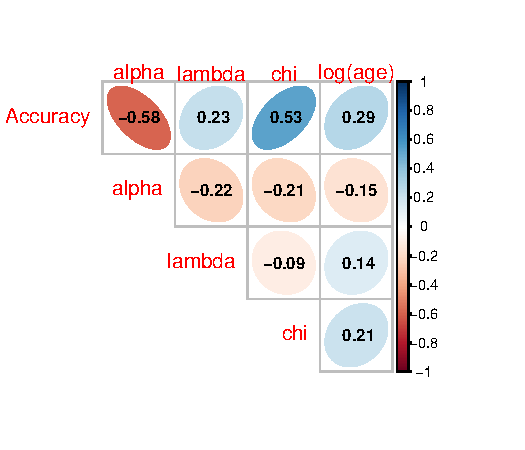
\includegraphics{figs/unnamed-chunk-2-1} \caption[Correlation of best-fitting model parameters]{Correlation of best-fitting model parameters}\label{fig:unnamed-chunk-2}
\end{figure}
\end{CodeChunk}

\begin{CodeChunk}
\begin{figure}[H]

{\centering 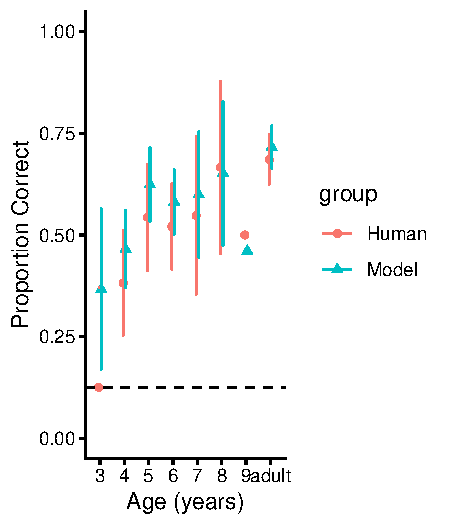
\includegraphics{figs/fig1-perf-1}

}

\caption[Model vs]{Model vs. human performance by age.}\label{fig:fig1-perf}
\end{figure}
\end{CodeChunk}

\subsection{Selection strategies}\label{selection-strategies}

The most likely selection strategy for each participant was calculated.
Confirmatory was the most common strategy (42\% of participants),
followed by entropy (29\%), margin sampling (18\%), random (8\%), and
novelty (3\%). Adults were more likely to use entropy maximization (39\%
vs.~20\% of children), whereas children were more likely to use a
confirmatory strategy (62\% vs.~22\% of adults). Margin sampling was
used at a similar rate by children (14\%) and adults (22\%), and a
random selection was most likely for 13\% of adults, but only 3\% of
children. Novelty was the most likely strategy for only 5\% of adults,
and was not used by any children.

\subsection{Relative contributions of strategy, age, and learning
mechanisms}\label{relative-contributions-of-strategy-age-and-learning-mechanisms}

To assess the relative importance of sampling strategy versus learning
mechanisms in predicting performance, we fitted a series of nested
regression models. A model including only sampling strategy explained
minimal variance in test accuracy (\(R^2 = .02\), F(4,185) = 0.94,
\(p=0.44\)). Adding age modestly improved the model (\(R^2 = 0.12\),
\(\beta = 0.15\), F(5,183) = 4.90, \(p<.001\)). A model including
sampling strategy and learning parameters (\(\chi\), \(\lambda\),
\(\alpha\)) explained much more variance (\(R^2 = 0.55\)), demonstrating
that individual differences in learning mechanisms vastly outweigh
strategy choice in determining learning success. Within the parameter
model, learning rate (\(\chi\): \(\beta = 0.35\), \(p < .001\)), memory
decay (\(\alpha\): \(\beta = -0.70\), \(p < .001\)), and attention to
uncertainty (\(\lambda\): \(\beta = 0.01\), \(p = .002\)) were
significant predictors, and one sampling strategy effect emerged:
information gain (entropy) was better than confirmatory sampling
(\(\beta = 0.08\), \(p=.03\)) Notably, age effects were fully mediated
by learning parameters: when they were included, age no longer predicted
performance (\(\beta = 0.04\), \(p = .17\)). This suggests that
developmental improvements in word learning operate primarily through
changes in learning rate and memory, rather than through strategy
sophistication or other age-related factors.

\begin{table}[H]
\centering
\begin{tabular}{lrr}
  \hline
strategy & n & proportion \\
  \hline
confirmatory &  81 & 0.42 \\
  entropy &  56 & 0.29 \\
  margin &  34 & 0.18 \\
  random &  15 & 0.08 \\
  novelty &   5 & 0.03 \\
   \hline
\end{tabular}
\caption{Most likely selection strategies.}
\end{table}

\begin{CodeChunk}
\begin{figure}[tb]
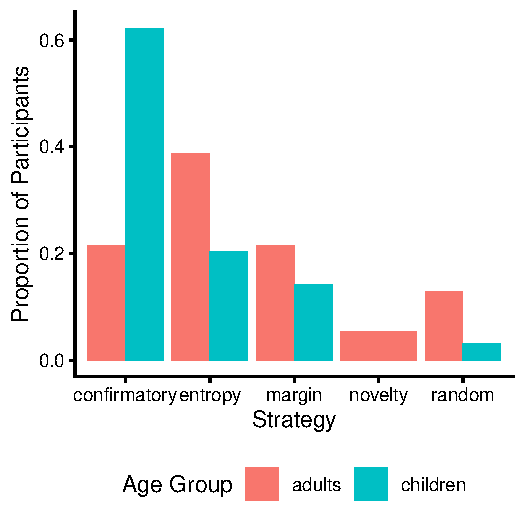
\includegraphics{figs/unnamed-chunk-7-1} \caption[Best-fitting selection strategies by age group]{Best-fitting selection strategies by age group.}\label{fig:unnamed-chunk-7}
\end{figure}
\end{CodeChunk}

\section{Discussion}\label{discussion}

We investigated the computational mechanisms underlying active word
learning by fitting associative learning models to individual
participants' performance and analyzing their information-seeking
strategies. Two models with uncertainty-biased attention best explained
learning for nearly all participants, with an uncertainty-only model
(UAM) best accounting for 51\% of individuals and the combined
familiarity-uncertainty model (FUAM) accounting for 48\%. This suggests
that directing attention toward uncertain associations (i.e., items with
diffuse mappings) is a fundamental mechanism in cross-situational word
learning in both adults and children. These two models -- differing only
in whether the current association strength is considered in the update
rule -- very nearly mimicked each other for the bulk of the participants
(X\%), but each model best explained a substantial group of
participants, suggesting some individual variability in learning styles.
Examining the best-fitting parameters showed that learning rate and
memory decay predicted performance more strongly than attention biases.
Participants with higher learning rates (\(\chi\)) and lower memory
fidelity (\(\alpha\); effectively forgetting early ambiguous evidence)
were more accurate at test. A relatively weak relationship between
\(\lambda\) (attention to uncertainty) and performance (\(r = 0.23\))
suggests that how much learners encode matters more than what they
attend to, at least in these experimental paradigms.

An analysis of selection strategies showed striking developmental
differences. Adults predominantly employed entropy maximization (39\%),
actively seeking information about ambiguous items to reduce
uncertainty. In contrast, children favored confirmatory sampling (62\%),
requesting information about items for which they already had strong
associations. This pattern suggests that uncertainty-reduction
strategies emerge gradually across development, consistent with broader
findings on the development of information-seeking in childhood (Meder
et al., 2021; Nussenbaum et al., 2019).

This could be due to a variety of reasons, including that children's
limited working memory doesn't allow them to effectively evaluate
multiple competing associations per item, or because they lack the
metacognitive awareness that a strategy of reducing uncertainty would be
beneficial. In contrast, a confirmatory sampling strategy can be
conducted even if a learner tracks only their strongest hypothesis.

A central theoretical question is whether sampling ambiguous items
causes better learning, or whether successful learning enables more
sophisticated sampling strategies. Our results support the latter
interpretation. Learning parameters \(\chi\) and \(\alpha\) strongly
predicted performance, while sampling strategy showed weaker
relationships to outcomes. Moreover, children (who learn less
successfully, overall) predominantly used confirmatory rather than
uncertainty-reducing strategies. This finding aligns with Zettersten \&
Saffran (2021)'s supplementary analysis which suggested that
``successfully learning novel words during training makes it more likely
that learners will subsequently focus on ambiguous items.'' We extend
this by showing that individual differences in learning mechanisms
(learning rate, memory) are the primary drivers of both performance and
sampling sophistication. Of course, the experimental design limits our
ability to test causality: selection trials occurred \emph{after}
initial learning, and we modeled them using associations built during
passive training. Future work using trial-by-trial joint optimization of
learning and selection parameters could better disentangle these
relationships.

Combining computational modeling of learning mechanisms with analysis of
selection strategies reveals a nuanced picture of active word learning
across development. Successful learning depends more on fundamental
learning parameters (i.e., how quickly associations form and how readily
early evidence is forgotten) rather than a bias to attend more or less
to uncertain (or already-familiar) items. However, the likelihood of
strategically sampling uncertain information emerges across childhood,
which may suggest an increasing awareness of uncertainty, or of the
value of reducing it. These findings advance our understanding of how
learners actively shape their own language learning experience, and how
cognitive development enables increasingly sophisticated
information-seeking strategies.

\section{Acknowledgements}\label{acknowledgements}

Place acknowledgments (including funding information) in a section at
the end of the paper.

\section{References}\label{references}

\setlength{\parindent}{-0.1in}
\setlength{\leftskip}{0.125in}

\noindent

\phantomsection\label{refs}
\begin{CSLReferences}
\bibitem[\citeproctext]{ref-gelderloos_active_2020}
Gelderloos, L., Mahmoudi Kamelabad, A., \& Alishahi, A. (2020). Active
word learning through self-supervision. In S. Denison, M. Mack, Y. Xu,
\& B. C. Armstrong (Eds.), \emph{Proceedings for the 42nd {Annual}
{Meeting} of the {Cognitive} {Science} {Society}} (pp. 1050--1056).
Cognitive Science Society.

\bibitem[\citeproctext]{ref-gureckis2012self}
Gureckis, T. M., \& Markant, D. B. (2012). Self-directed learning: A
cognitive and computational perspective. \emph{Perspectives on
Psychological Science}, \emph{7}(5), 464--481.

\bibitem[\citeproctext]{ref-hembacher_childrens_2020}
Hembacher, E., DeMayo, B., \& Frank, M. C. (2020). Children's social
information seeking is sensitive to referential ambiguity. \emph{Child
Development}, \emph{91}(6), e1178--e1193.
http://doi.org/\href{https://doi.org/10.1111/cdev.13427}{10.1111/cdev.13427}

\bibitem[\citeproctext]{ref-Hidaka2017}
Hidaka, S., Torii, T., \& Kachergis, G. (2017). Quantifying the impact
of active choice in word learning. In G. Gunzelmann, A. Howes, T.
Tenbrink, \& E. Davelaar (Eds.), \emph{Proceedings of the 39th {Annual}
{Meeting} of the {Cognitive} {Science} {Society}} (pp. 519--525).
Austin, TX: Cognitive Science Society.

\bibitem[\citeproctext]{ref-Kachergis2013}
Kachergis, George, Yu, C., \& Shiffrin, R. M. (2013). Actively learning
object names across ambiguous situations. \emph{Topics in Cognitive
Science}, \emph{5}(1), 200--13.
http://doi.org/\href{https://doi.org/10.1111/tops.12008}{10.1111/tops.12008}

\bibitem[\citeproctext]{ref-Kachergis2017}
Kachergis, G., Yu, C., \& Shiffrin, R. M. (2016). A bootstrapping model
of frequency and contextual diversity effects in word learning.
\emph{Cognitive Science}, \emph{41}(3).

\bibitem[\citeproctext]{ref-Kachergis2012}
Kachergis, Y., G. (2012). An associative model of adaptive inference for
learning word--referent mappings. \emph{Psychonomic Bulletin and
Review}, \emph{19}(2), 317--324.

\bibitem[\citeproctext]{ref-Keijser2019}
Keijser, D., Gelderloos, L., \& Alishahi, A. (2019). Curious topics: {A}
curiosity-based model of first language word learning. In
\emph{Proceedings of the 41st {Annual} {Conference} of the {Cognitive}
{Science} {Society}} (pp. 1991--1997). Montreal, QB: Cognitive Science
Society.

\bibitem[\citeproctext]{ref-markant2016}
Markant, D. B., Settles, B., \& Gureckis, T. M. (2016). Self-directed
learning favors local, rather than global, uncertainty. \emph{Cognitive
Science}, \emph{40}(1), 100--120.
http://doi.org/\href{https://doi.org/10.1111/cogs.12220}{10.1111/cogs.12220}

\bibitem[\citeproctext]{ref-meder_directed_2021}
Meder, B., Wu, M. C., Schulz, E., \& Ruggeri, A. (2021).
\href{https://www.ncbi.nlm.nih.gov/pubmed/25246403}{Directed and random
exploration in children}. \emph{Preprint}.

\bibitem[\citeproctext]{ref-Nelson2005}
Nelson, J. D. (2005). Finding useful questions: {On} {Bayesian}
diagnosticity, probability, impact, and information. \emph{Psychological
Review}, \emph{112}(4), 979--999.

\bibitem[\citeproctext]{ref-nelson_experience_2010}
Nelson, J. D., McKenzie, C. R. M., Cottrell, G. W., \& Sejnowski, T. J.
(2010). Experience {Matters}: {Information} {Acquisition} {Optimizes}
{Probability} {Gain}. \emph{Psychological Science}, \emph{21}(7),
960--969.
http://doi.org/\href{https://doi.org/10.1177/0956797610372637}{10.1177/0956797610372637}

\bibitem[\citeproctext]{ref-nussenbaum_causal_2019}
Nussenbaum, K., Cohen, A. O., Davis, Z., Halpern, D., Gureckis, T., \&
Hartley, C. (2019). Causal information-seeking strategies change across
childhood and adolescence,\emph{ April 12}, 1--18.
http://doi.org/\href{https://doi.org/10.31234/OSF.IO/QUKAC}{10.31234/OSF.IO/QUKAC}

\bibitem[\citeproctext]{ref-nussenbaum_novelty_2023}
Nussenbaum, K., Martin, R. E., Maulhardt, S., Yang, Y. J.,
Bizzell-Hatcher, G., Bhatt, N. S., \ldots{} Cockburn, J. (2023). Novelty
and uncertainty differentially drive exploration across development.
\emph{Elife}, \emph{12}, e84260. Retrieved from
\url{https://elifesciences.org/articles/84260}

\bibitem[\citeproctext]{ref-Settles2012}
Settles, B. (2012). \emph{Active {Learning}} (Vol. 6).
http://doi.org/\href{https://doi.org/10.2200/S00429ED1V01Y201207AIM018}{10.2200/S00429ED1V01Y201207AIM018}

\bibitem[\citeproctext]{ref-smith2018developing}
Smith, L. B., Jayaraman, S., Clerkin, E., \& Yu, C. (2018). The
developing infant creates a curriculum for statistical learning.
\emph{Trends in Cognitive Sciences}, \emph{22}(4), 325--336.

\bibitem[\citeproctext]{ref-twomey2018curiosity}
Twomey, K. E., \& Westermann, G. (2018). Curiosity-based learning in
infants: A neurocomputational approach. \emph{Developmental Science},
\emph{21}(4), e12629.

\bibitem[\citeproctext]{ref-wason1960}
Wason, P. C. (1960). On the failure to eliminate hypotheses in a
conceptual task. \emph{Quarterly Journal of Experimental Psychology},
\emph{12}(3), 129--140.

\bibitem[\citeproctext]{ref-woodard2016}
Woodard, K., Gleitman, L. R., \& Trueswell, J. C. (2016). Two-and
three-year-olds track a single meaning during word learning: Evidence
for propose-but-verify. \emph{Language Learning and Development},
\emph{12}(3), 252--261.

\bibitem[\citeproctext]{ref-yu2007rapid}
Yu, C., \& Smith, L. B. (2007). Rapid word learning under uncertainty
via cross-situational statistics. \emph{Psychological Science},
\emph{18}(5), 414--420.

\bibitem[\citeproctext]{ref-zettersten_active_2023}
Zettersten, M., Cutler, M., \& Lew-Williams, C. (2023). \emph{Active
information-seeking in support of learning extensions of novel words}
(preprint). PsyArXiv. Retrieved from \url{https://osf.io/ecq85}

\bibitem[\citeproctext]{ref-Zettersten2021}
Zettersten, M., \& Saffran, J. R. (2021). Sampling to learn words:
Adults and children sample words that reduce referential ambiguity.
\emph{Developmental Science}, \emph{24}(3).
http://doi.org/\href{https://doi.org/10.1111/desc.13064}{10.1111/desc.13064}

\end{CSLReferences}




\end{document}
